\hsection{Search Spaces and Encodings}%
\label{sec:searchSpace}%
%
The solution space~\solutionSpace\ is the data structure that \inQuotes{makes sense} from the perspective of the user, the decision maker, who will be supplied with one instance of this structure (a candidate solution~\solspel) at the end of the optimization procedure.
But~\solutionSpace\ not necessarily is the space that is most suitable for searching inside.

We have already seen that there are several constraints that apply to the Gantt charts.
For every problem instance, different solutions may be feasible.
Besides the constraints, the space of Gantt charts also looks kind of unordered, unstructured, and messy.

Let's say that we want to generate a valid Gantt chart for a \gls{JSSP} instance.
We would step-by-step fill the Gantt chart by placing the different operations in the right order, without adding useless waiting times.
Now if we wanted to take a feasible Gantt chart and try to tweak it in some way, we begin getting into trouble.
If we did not insert useless waiting times, then each operation occurs at the earliest time where it can be placed based on all previously assigned operations.
Thus, to move an operation around, we would first need to try to swap and move some previous operations.
And then, if we succeeded somehow and the operation now indeed is moved to earlier time, we would need to move all the operations that come after it forward as well.
During all of this, we need to keep track of the instance data~\instance\ to not accidentally violate some constraint.
Thus, while we do have found a reasonable representation of solutions for the \gls{JSSP} in Gantt charts, it is only really suitable to represent single, fixed solutions.
It is not really suitable to explore a space~\solutionSpace\ of different solutions -- at least unless we are willing to write complicated code dealing with the feasibility constraints.

Actually, many data structures that represent real-world objects with their features, be it Gantt charts, construction plans of airplane wings, or plans for electronic circuits are specialized and do not lend them themselves to be directly processed by general algorithms.

It would thus be nice to have a compact, clear, and easy-to-understand way to explore different candidate solutions.
Something that we can instantiate and modify in a simple way without getting in trouble%
%
\hsection{Definitions}%
%
\begin{definition}[Search Space]%
\label{def:searchSpace}%
The \emph{search space}~\searchSpace\ is a representation of the solution space~$\solutionSpace$ suitable for exploration by an algorithm.%
\end{definition}%
%
\begin{definition}[Point in the Search Space]%
\label{def:searchSpacePoint}%
The elements~$\sespel\in\searchSpace$ of the search space~\searchSpace\ are called \emph{points} in the search space.%
\end{definition}%
%
\begin{definition}[Decoding Function]%
\label{def:decoding}%
The \emph{decoding function}~$\decode:\searchSpace\mapsto\solutionSpace$ is a left-total relation which maps each point~$\sespel\in\searchSpace$ of the search space~\searchSpace\ to one candidate solution~$\solspel\in\solutionSpace$ in the solution space~\solutionSpace.%
\end{definition}%
%
\inQuotes{Left-total} here means that every point in~\searchSpace\ is mapped to one point in~\solutionSpace.
Some points in~\searchSpace\ may be mapped to the same point in~\solutionSpace.
There even may be some points in~\solutionSpace\ for which no corresponding point in~\searchSpace\ exists.%
%
\begin{definition}[Representation, Encoding]%
\label{def:encoding}%
The solution space~\solutionSpace, search space~\searchSpace, and the decoding function~\decode\ together are called the \emph{encoding} or the \emph{representation}.%
\end{definition}%
%
The solution space~\solutionSpace\ is what the user cares about.
The optimization algorithm, however, \emph{only} works on the search space~\searchSpace.
It does not need to know or care about what the candidate solutions are.
The candidate solutions can be complex structures, such as the shape of the nose of a fast train~\cite{IMNFM1997ENSFRTSB,KIF2011OOTNSFRMPWRFTE}.
It is hard to imagine how to search inside the space of all possible such shapes in a targeted way.
However, maybe we could encode the surfaces of the train noses as vectors of real numbers.
The search space could then just be an $n$\nobreakdash-dimensional real vector space.
This changes everything.
We know and understand these vector spaces since high school.
We have all kinds of tools available to search in it in an ordered fashion, ranging from distance metrics to vector mathematics.
Suddenly, the problem becomes easier to approach algorithmically.
Moreover, since real vector spaces are very common, there already exists a wide variety of algorithms that can perform optimization over them.

A good encoding, i.e., a suitable search space~\searchSpace\ and mapping~$\decode:\searchSpace\mapsto\solutionSpace$ can make our life much easier.

For applying an optimization algorithm, we therefore usually choose a data structure~\searchSpace\ which we can understand intuitively.
Ideally, it should be possible to define concepts such as distances, similarity, or neighborhoods on this data structure.
Spaces that are especially suitable for searching in include, for example:%
%
\begin{enumerate}%
%
\item subsets of $n$\nobreakdash-dimensional real vectors, i.e., $\realNumbers^n$,%
%
\item the set of all possible permutations of~$n$ objects, and%
%
\item a number of~$n$ yes-no decisions, which can be represented as bit strings of length~$n$, spanning the space~$\{0,1\}^n$.%
%
\end{enumerate}%
%
For such spaces, we can relatively easily define good search methods and can rely on a large amount of existing research work and literature.
If we are lucky, then our solution space~\solutionSpace\ is already \inQuotes{similar} to one of these well-known and well-researched data structures.
Then, we can set~$\searchSpace=\solutionSpace$ and use the identity mapping~$\decodeOf{\sespel}=\sespel\;\forall \sespel\in\searchSpace$ as decoding function.
In other cases, we will often prefer to map~\solutionSpace\ to something similar to these spaces and define~\decode\ accordingly.

The mapping~\decode\ does not need to be injective, as it may map two points~$\sespel_1$ and~$\sespel_2$ to the same candidate solution even though they are different~($\sespel_1\neq\sespel_2$).
Then, there exists some redundancy in the search space.
We would normally like to avoid redundancy, as it tends to slow down the optimization process~\cite{KW2002OTUOREIMBES}.
Being injective is therefore a good feature for~\decode.

The mapping~\decode\ also does not necessarily need to be surjective, i.e., there can be candidate solutions~$\solspel\in\solutionSpace$ for which no~$\sespel\in\searchSpace$ with $\decodeOf{\sespel}=\solspel$ exists.
However, such solutions then can never be discovered.
If the optimal solution would be among those unreachable ones, then, well, it could not be found by the optimization process.
Being surjective is therefore a good feature for~\decode.

Finally, and as a side note:
Technically speaking, \decode\ does not even necessarily be a function.
It could be a randomized procedure, meaning that two invocations could lead to different results.
But let's not take things too far here.%
%
\endhsection%
%
\hsection{A Programmer's Perspective}%
%
In \cref{lst:Space}, we already have defined a simple API to provide common operations for (solution) spaces.
We can reuse this very same API for search spaces too.
Additionally, we need a function that can convert from points in the search space to candidate solutions.%
%
\moptipyCode{moptipy/api/encoding.py}{--labels book --args doc}{Encoding}{A base class for encodings.}%

The class given in \cref{lst:Encoding} provides the blueprint for a function \codeil{decode} which translates one point~\codeil{x} in the search space to a candidate solution instance~\codeil{y} of the solution space.
This \codeil{decode} function corresponds to the general definition~$\decode:\searchSpace\mapsto\solutionSpace$ of the encoding.
An implementation of \codeil{decode} will overwrite whatever contents were stored in the object~\codeil{y}, i.e., we assume the objects~\codeil{y} can be modified.

Thus, if you want to use a certain search space~\searchSpace\ and a different solution space~$\solutionSpace\neq\searchSpace$, you would provide an encoding~$\decode:\searchSpace\mapsto\solutionSpace$ by deriving a new class from \codeil{Encoding} and implementing \decode\ as \codeil{decode}.
The optimization algorithm can then search in the simple space~\searchSpace\ whereas the user and the objective function~\objf\ only get to see the candidate solutions~$\solspel\in\solutionSpace$.
This is possible because between these two components, the decoding function~\decode\ translates the points~$\sespel\in\searchSpace$ generated by the optimization algorithm to the candidate solutions in~\solutionSpace.%
%
\endhsection%
%
\hsection{Example: Job Shop Scheduling}%
\label{sec:jsspSearchSpace}%
%
In our \gls{JSSP} example problem, the candidate solutions are Gantt charts.
We developed the class \codeil{Gantt} given in \cref{lst:jssp_gantt} to represent their data.
This data can easily be interpreted and visualized by the user.
Yet, it is not that clear how we can efficiently create such solutions, especially feasible ones, let alone how to \emph{search} in the space of Gantt charts.\footnote{%
Of course, there are many algorithms that can do that and we could design one such algorithm if we would seriously think about it, but here we take the educational route where we investigate the full scenario with~$\searchSpace\neq\solutionSpace$.} %
What we would like to have is a \emph{search space}~\searchSpace, which can represent the possible candidate solutions of the problem in a more machine-tangible, algorithm-friendly way.

The \gls{JSSP} is a very well-known problem.
Comprehensive overviews about different such search spaces for the \gls{JSSP} can be found in~\cite{CGT1996ATSOJSSPUGAIR,W2013GAFSSPAS,A2010RIGAFTJSPACS,YN1997GAFJSSP}.
We here will develop only one single idea which I find particularly appealing.%
%
\hsection{Idea: 1-dimensional Encoding}%
%
Imagine you would like to construct a Gantt chart as candidate solution for a given \gls{JSSP} instance.
How would you do that?
Well, we know that each of the $\jsspJobs$~jobs has $\jsspMachines$~operations, one for each machine.
We could simply begin by choosing one job and placing its first operation on the machine to which it belongs, i.e., write it into the Gantt chart.
Then we again pick a job, take the first not-yet-scheduled operation of this job, and \inQuotes{add} it to the end of the row of its corresponding machine in the Gantt chart.
Of course, we cannot pick a job whose operations all have already be assigned.
We can continue doing this until all operations of all jobs are assigned.
The result will be a \emph{feasible} solution.

This feasible solution is defined by the order in which we chose the jobs.
Such an order can be described as a simple, linear string of job~IDs, i.e., of integer numbers.
Each job~ID would appear \jsspMachines~times, because that is how many operations the job has.
We would process such a string from the beginning to the end.
Whenever encountering a job~ID, we assign the first not-yet assigned operation of the job to its correspoinding machine.
We will always get a feasible Gantt chart as result.
It is not possible to produce a deadlock (see \cref{sec:solutionSpace:feasibility}), because we will only allocate an operation to a machine after having placed all operations that come before it in the same job.

\begin{figure}%
\centering%
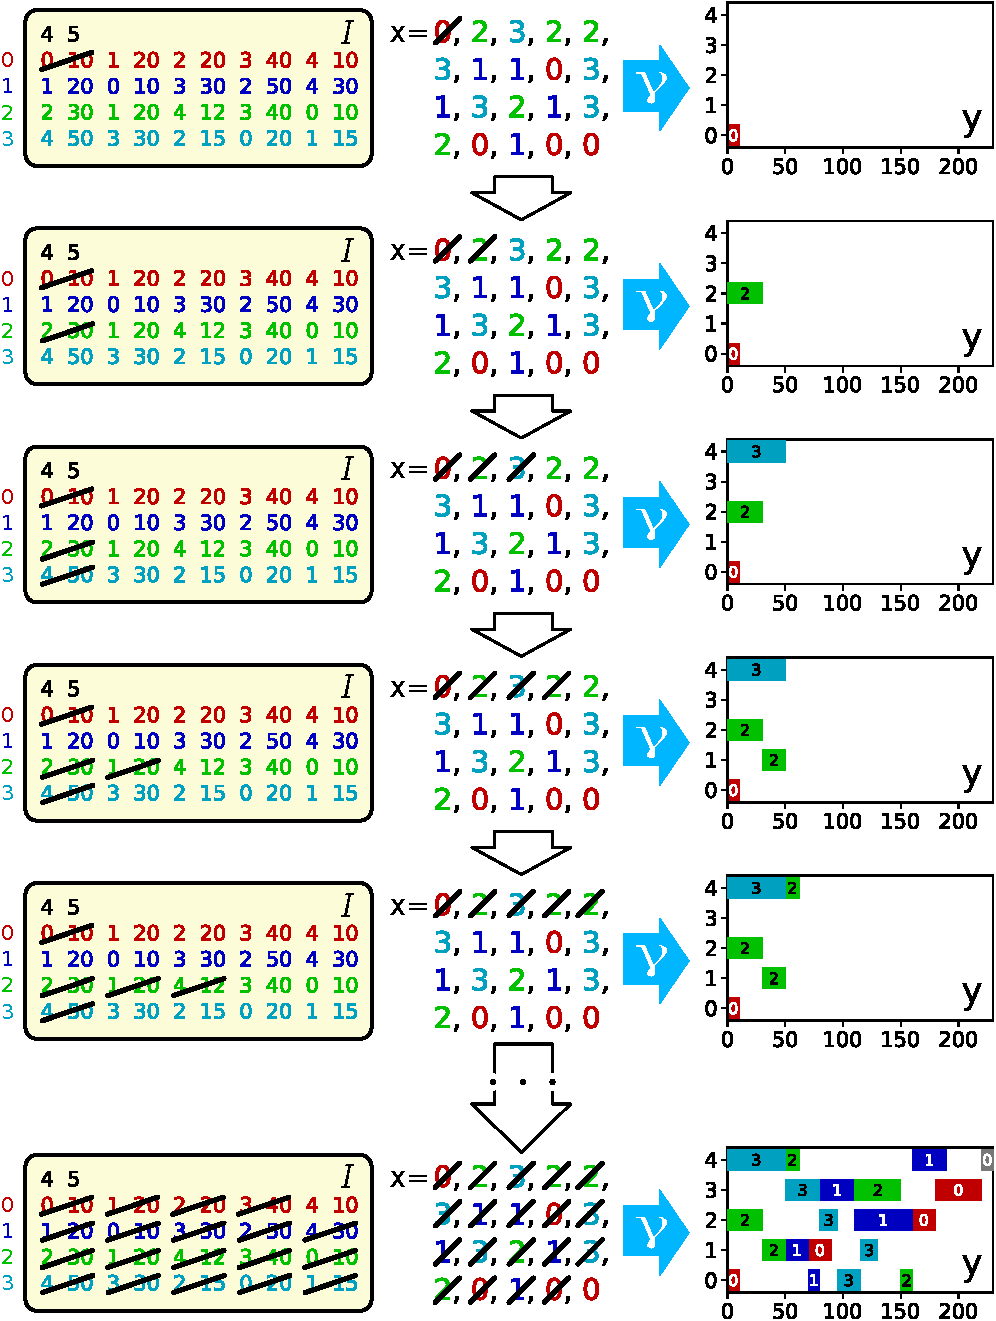
\includegraphics[width=0.97\linewidth]{\currentDir/jssp_encoding.pdf}%
\caption{Illustration of the first five steps and the second-to-last step of the decoding of an example point in the search space to a candidate solution.}%
\label{fig:jssp_encoding}%
\end{figure}

This decoding procedure can best be described by an example.
In the \instStyle{demo} instance, we have $\jsspMachines=5$~machines and $\jsspJobs=4$~jobs.
Each job thus has $\jsspMachines=5$~operations that must be assigned to the machines.
We use an integer string~\sespel\ of length~$\jsspMachines*\jsspJobs=20$ denoting the priority of the operations.
We \emph{know} the order of the operations per job as part of the problem instance data~\instance.
We therefore do not need to store it in the string~\sespel.
We just include the ID of each job $\jsspMachines=5$~times in the string.

The encoding represents the order in which we assign the $\jsspJobs$~jobs, and each job must be picked $\jsspMachines$~times.
Our search space is thus somehow similar to the set of permutations of~$\jsspJobs*\jsspMachines$ objects mentioned earlier, but instead of permutations, we have \emph{permutations with repetitions}.

A point~$\sespel\in\searchSpace$ in the search space~$\searchSpace$ for the \instStyle{demo} \gls{JSSP} instance would thus be an integer string of length~20.
As example, we choose $\sespel=(0, 2, 3, 2, 2, 3, 1, 1, 0, 3, 1, 3, 2, 1, 3, 2, 0, 1, 0, 0)$.

Let us now exercise the decoding procedure~\decodeOf{\sespel}.
In \cref{fig:jssp_encoding}, we sketch several of its steps.
For each step, we show the instance data~\instance\ on the left, the point~\sespel\ in the search space in the middle, and the current state of the Gantt chart~\solspel\ on the right hand side.

The decoding of the string~\sespel\ starts with an empty Gantt chart.
This string is interpreted from left to right, as illustrated in the figure.
The first value is~0, which means that, in the first step, job~0 is assigned to a machine.
From the instance data, we know that job~0 first must be executed for 10~time units on machine~0.
The job is thus inserted on machine~0 in the chart.
Since machine~0 is initially idle and thus immediately ready to be used, the operation can be placed at time index~0.
We also know that this operation can definitely be executed, i.e., won't cause a deadlock, because it is the first operation of the job.
Once we have placed it in the chart, we cross it out to mark it as assigned.
This happens in the first line in our figure.

The next value in the string is~2, meaning that we now need to insert an operation from job~2.
No operation from this job was processed yet, so we pick its first operation.
From the instance data, we see that it should go to machine~2 for 30~time units.
In our current Gantt chart, no job has yet been assigned to machine~2, so we can place it there at time index~0.
We now cross out this operation as well.
This is done in the second line of the figure.

We then encounter the value~3 in the string for the first time.
Job~3 first goes to machine~4 for 50~time units.
Machine~4 is still unused, so we can place it there directly and mark it as assigned, as shown in line~3 of our figure.

Next we encounter job~2 again, i.e., for the second time.
We have already marked its first operation as assigned.
So we now need to allocate its second operation.
It should go to machine~1 for 20~time units.
While machine~1 has no job assigned to it yet, we cannot place the operation at time index~0.
We first need to wait for the first operation of job~2 to complete, which happens at time index~30.
Hence, we can start the operation at that time.

In the fifth row of \cref{fig:jssp_encoding}, we again find job~2.
We need to assign its third operation, which goes to machine~4 and will need 12~time units there.
It can only start after the second operation of the job is completed, which happens after $30+20=50$~time units.
Also, machine~4 is used by job~3, whose first operation will be completed there also after 50~time units.
Therefore, the third operation of job~2 can begin there at time index~50.

We then again encounter job~3 in~\sespel, which means we need to assign its second operation.
This operation goes to machine~3 and can start at time index~50, after the first operation of the job has been completed.
Then we will encounter job~1 for the first time and allocate its first operation to machine~1 for 20~time units.
It can start after the second operation of job~2, which is already assigned to that machine, completes, i.e., at time index~50.\footnote{%
The reader will notice: %
Actually, we could let it start at time index~0, which would not interfere with the operation of job~2. %
However, this would make the mapping more complicated, so we stick to the easier approach of just adding it at the end here.}
Directly afterwards, job~1 needs to be assigned again and its second operation will go to machine~0.
It can start at time index~$50+20=70$, namely after its first operation is completed.

We continue this iterative process.
The last row of \cref{fig:jssp_encoding} illustrates the second-to-last decoding step.
It places the second-to-last operation of job~0 onto machine~3.
The previous (i.e., third) operation of the job was on machine~2 and completed there after 180~time units.
Machine~3 is idle at that time, so operation~4 of job~1 will occupy it from time index~180 to~220.
This only leaves only the last operation of job~1 to be assigned, which will take~10 time units on machine~4.
It can start there directly at time index~220 and will finish on time index~230 (illustrated in dark gray in the figure).

The Gantt chart then is complete.
Whenever we assigned a operation~$\jsspJobIndex>0$ of any given job to a machine, then we already had assigned all operations at smaller indices first.
No deadlock can occur and~\solspel\ must therefore be feasible.

\moptipyCode{moptipy/examples/jssp/ob_encoding.py}{--labels book --args comments,doc}{jssp_encoding}{An excerpt of the implementation of the operation-based encoding for the \gls{JSSP}.}

In \cref{lst:jssp_encoding}, we illustrate how such an encoding can be implemented.
It basically is a function translating an \numpyndarray\ of integers to a \codeil{Gantt} chart.
We put the algorithm into a function \codeil{decode}, so that we can mark it for compilation with \numba\ to improve the performance, utilizing the performance tips discussed in TODO.

\moptipyCode{moptipy/spaces/permutations.py}{--labels book --args doc,comments}{PermutationsWithRepetitions}{Excerpt of the implementation of the \codeil{Space} API from \cref{lst:Space} for permutations with (or without) repetitions.}

Besides implementing the decoding function~\decode, we also need to provide the functionality of our \codeil{Space} API for (search) spaces that are permutations with repetitions.
This functionality will be needed to create, copy, store, load, and check the points in the search space.
In \cref{lst:PermutationsWithRepetitions}, we provide a very small excerpt of the implementation of the \codeil{Space} API for permutations of numbers stored in \numpyndarrays.
This class is quite general:
We provide a \codeil{blueprint} string of the numbers that we want to arrange in the permutations.
This could be a true permutation, e.g., $[1, 2, 3]$, or a permutation with repetitions, such as $[1, 1, 2, 2, 3, 3]$.
The \codeil{create} method of the \codeil{Space} implementation will always return a copy of that blueprint array.
We omit the conversion to and from text strings, as it can be implemented similarly as in \codeil{lst:jssp_gantt_space}.
Validation can simply check whether each job ID occurs exactly as needed, i.e., $\jsspMachines$~times in our case, and is thus also not printed.
The static method \codeil{with_repetitions} instantiates the space for \jsspMachines~repetitions of the elements~\intRange{0}{\jsspJobs-1}.%
%
\endhsection%
%
\hsection{Advantages of this very simple Encoding}%
%
We now have a natural way to represent Gantt charts with a much simpler data structure.
Because this method is so intuitive, it has been discovered by several researchers independently, the earliest being \citeauthor{GTK1994SJSSPBGA}~\cite{GTK1994SJSSPBGA}, \citeauthor{B1995AGPATJSSWGA}~\cite{B1995AGPATJSSWGA,BMK1996OPRFSP}, and \citeauthor{SIS1997NESFSJSPBGA}~\cite{SIS1997NESFSJSPBGA}, all in the 1990s.

But what do we gain by using this encoding?

Well, we now have a very simple data structure~\searchSpace\ to represent our candidate solutions.
It is much simpler than the Gantt charts.
It is just a linear sequence of \jsspJobs~numbers, each occuring a fixed amount~\jsspMachines\ of times.

As a direct result, we also have very simple rules for validating a point~$\sespel\in\searchSpace$ in the search space:
If it contains the numbers~$\intRange{0}{(\jsspJobs-1)}$ each exactly~$\jsspMachines$ times, it represents a feasible candidate solution.

The candidate solution corresponding to a valid point from the search space will always be \emph{feasible}~\cite{B1995AGPATJSSWGA}.
The mapping~\decode\ will ensure that the order of the operations per job is always observed.
Thus, we have solved the issue of deadlocks mentioned in \cref{sec:solutionSpace:feasibility}.
We know from \cref{tbl:jsspSolutionSpaceFeasibleTable}, that the vast majority of the possible Gantt charts for a given problem might actually be infeasible.
Now we do no longer need to worry about that.
Our mapping~\decode\ also obeys the more trivial constraints, such as that each machine will process at most one job at a time and that all operations are eventually processed.

Finally, we also could modify our decoding function~\decode\ to adapt to more complicated and constraint versions of the \gls{JSSP} if need be:
For example, imagine that it would take a job- and machine-dependent amount of time for carrying a the material produced by on job from the current machine to the next machine.
We could easily facilitate this by changing~\decode\ by adding this time to the starting time of the job.
If there was a job-dependent setup time for each machine~\cite{ANCK2008ASOSPWSTOC}, which could be different if job~1 follows job~0 instead of job~2, then this could be facilitated easily as well.
If our operations would be assigned to \inQuotes{machine types} instead of \inQuotes{machines} and there could be more than one machine per machine type, then the representation mapping could assign the operations to the next machine of their type which becomes idle.
Our representation also trivially covers the situation where each job may have more than~\jsspMachines\ operations, i.e., where a job may need to cycle back and pass one machine twice.
It is also suitable for simpler scenarios, such as the \acrfull{FSSP}, where all jobs pass through the machines in the same, pre-determined order~\cite{T1993BFBSP,GJS1976TCOFAJS,W2013GAFSSPAS}.

Many such different problem flavors can now be reduced to investigating the same space~\searchSpace\ using the same optimization algorithms, just with slightly different decoding function~\decode\ and/or objective functions~\objf.
Additionally, it becomes  easy to indirectly create and modify candidate solutions by sampling points from the search space and moving to similar points, as we will see in the following chapters.
\endhsection%
%
\hsection{Size of the Search Space}%
\label{sec:size_of_jssp_search_space}%
%
It is relatively easy to compute the size~$\left|\searchSpace\right|$ of our proposed search space~\searchSpace~\cite{SIS1997NESFSJSPBGA}.
We do not need to make any assumptions regarding \inQuotes{no useless waiting time}, as in \cref{sec:solutionSpace:size}, since useless delays cannot occur by default.
Each element~$\sespel\in\searchSpace$ is a permutation of a multiset where each of the \jsspJobs~elements occurs exactly \jsspMachines~ times.
This means that the size of the search space can be computed as given in \cref{eq:jssp_search_space_size}.%
%
\begin{align}%
\left|\searchSpace\right| = \frac{\left(\jsspMachines*\jsspJobs\right)!}{ \left(\jsspMachines!\right)^{\jsspJobs} }%
\label{eq:jssp_search_space_size}%
\end{align}%
%
To better understand this equation, imagine the space of all permutations of the sequence $(1, 2, 3, 4)$.
Clearly there are $4!=4*3*2*1=24$ such permutations.
Now let us imagine that one number, say~$3$, appears twice, e.g., we want all the permutations of~$(1, 2, 3, 3, 4)$.
There are five elements now, so there are $5!=120$~possible ways to arrange them.
However, the number~$3$ appears twice and it does not matter which of the~$3$s appears first, so we get $5!/2=60$ possible unique permutations.
If we add another~$3$, i.e., $3$~would appear three times and we have~$(1, 2, 3, 3, 3, 4)$, then there would be $6!/3!=720/6=120$ possible arrangements.
If we now add another two~$4$s, we get $(1, 2, 3, 3, 3, 4, 4, 4)$.
This sequence can be arranged in $8!/(3!*3!)=40320/36=120$ possible ways.
If each one of \jsspJobs~different numbers appears \jsspMachines~times, we hence have $(\jsspJobs*\jsspMachines)/(\jsspMachines)^{\jsspJobs}$ different possible permutations, i.e., obtain \cref{eq:jssp_search_space_size}.

\begin{table}%
\centering%
\caption{The sizes~$\left|\searchSpace\right|$ and~$\left|\solutionSpace\right|$ of the search and solution spaces for selected values of the numbers of jobs~\jsspJobs\ and machines~\jsspMachines\ of a \gls{JSSP} instance~\instance.}%
\label{tbl:jsspSearchSpaceTable}%
%
\begin{booktabular}{lrrrr}%
example&\jsspJobs&\jsspMachines&$\left|\solutionSpace\right|$&$\left|\searchSpace\right|$\\%
\midrule%
&3&2&36&90\\%
&3&3&216&1\dgsep680\\%
&3&4&1\dgsep296&34\dgsep650\\%
&3&5&7\dgsep776&756\dgsep756\\%
&4&2&576&2\dgsep520\\%
&4&3&13\dgsep824&369\dgsep600\\%
&4&4&331\dgsep776&63\dgsep063\dgsep000\\%
\instStyle{demo}&4&5&7\dgsep962\dgsep624&11\dgsep732\dgsep745\dgsep024\\%
&5&2&14\dgsep400&113\dgsep400\\%
&5&3&1\dgsep728\dgsep000&168\dgsep168\dgsep000\\%
&5&4&207\dgsep360\dgsep000&305\dgsep540\dgsep235\dgsep000\\%
&5&5&24\dgsep883\dgsep200\dgsep000&$\approx6.234*10^{14}$\\%
\instStyle{orb06}&10&10&$\approx3.959*10^{65}$&$\approx2.357*10^{92}$\\%
\instStyle{la38}&15&15&$\approx5.591*10^{181}$&$\approx2.252*10^{251}$\\%
\instStyle{abz8}&20&15&$\approx6.193*10^{275}$&$\approx1.432*10^{372}$\\%
\instStyle{yn4}&20&20&$\approx5.278*10^{367}$&$\approx1.213*10^{501}$\\%
\instStyle{swv14}&50&10&$\approx6.772*10^{644}$&$\approx1.254*10^{806}$\\%
\instStyle{dmu72}&50&15&$\approx1.762*10^{967}$&$\approx3.862*10^{1\dgsep226}$\\%
\instStyle{dmu67}&40&20&$\approx1.710*10^{958}$&$\approx2.768*10^{1\dgsep241}$\\%
\instStyle{ta70}&50&20&$\approx4.587*10^{1\dgsep289}$&$\approx1.988*10{1\dgsep648}$\\%
\end{booktabular}%
\end{table}

We give some example values for this search space size~$\left|\searchSpace\right|$ in \cref{tbl:jsspSearchSpaceTable}.
From the table, we can immediately see that the number of points in the search space, too, grows very quickly with both the number of jobs~\jsspJobs\ and the number of machines~\jsspMachines\ of a \gls{JSSP} instance~\instance.
If we compare the ordering of our example \gls{JSSP} instances by search space size with the ordering by solution space, we find that there only is one disagreement:
\instStyle{dmu67} has the larger search space~\searchSpace\ but a smaller solution space~\solutionSpace\ compared to \instStyle{dmu72}.
Apart from this, larger solution spaces tend to correspond to larger search spaces as well.

For our \instStyle{demo} \gls{JSSP} instance with $\jsspJobs=4$~jobs and $\jsspMachines=5$~machines, we already have about 12~billion different points in the search space that represent 7~million possible non-wasteful candidate solutions.

We now find the drawback of our encoding:
There is much redundancy in our mapping.
The mapping~\decode\ is not injective.
Some elements of the search space~\searchSpace\ will map to the same element in the solution space~\solutionSpace.

For example, we could arbitrarily swap the first three numbers in the example string in \cref{fig:jssp_encoding} and would obtain the same Gantt chart, because jobs~0, 2, and~3 start at different machines.

As said before, we should avoid redundancy in the search space.
However, here we will stick with our proposed mapping because it is very simple, it solves the problem of feasibility of candidate solutions, and it allows us to relatively easily introduce and discuss many different approaches, algorithms, and sub-algorithms.%
\endhsection%
\endhsection%
%
\hsection{Summary}%
So far, we have focussed on elements that always must be present.
We have learned that a concrete set of input data for the optimization algorithms is called a problem instance~\instance.
We have learned that we need a data structure~\solutionSpace\ to represent candidate solutions~\solspel.
We have learned that we need an objective function~$\objf:\solutionSpace\mapsto\realNumbers$ that computes the cost of the candidate solutions (and that, usually, smaller values of~\objf\ indicate better solutions).

In this section, however, we have learned \emph{optional} components of the structure of optimization: the search space~\searchSpace\ and the decoding function~$\decode:\searchSpace\mapsto\solutionSpace$ that translates points~$\sespel\in\searchSpace$ to candidate solutions~$\solspel\in\solutionSpace$.
In many cases, neither~\searchSpace\ nor \decode\ are needed and we can search in~\solutionSpace\ as-is.
However, in many \emph{other} cases, the data structure~\solutionSpace\ that we can present to the user and rate with the objective function~\objf\ is not suitable to be explored directly during the optimization process.
It may either be too constraint or too complicated.

Then, we may come up with a way~\decode\ to translate some very simple space~\searchSpace, let's say bit strings, real vectors, or permutations to~\solutionSpace.
If we can do this, we immediately can reap several benefits:
Many algorithms that work well on such spaces already exist.
The spaces are simpler and it is easier to design search operators for them (we will learn later what that is).
Maybe we can even take care of some of the constraints during the mapping~\decode, as is the case in our \gls{JSSP} example.

Nevertheless, search space~\searchSpace\ and the decoding function~\decode\ are purely internal constructs.
They are meaningful \emph{only} for the optimization algorithm.
They are entirely meaningless for the user.
(Imagine handing a permutation with repetition as solution for a \gls{JSSP} to the human operator of a factory\dots)
They are also entirely meaningless from the perspective of the objective function~\objf.
Both the user and~\objf\ only are interested in the candidate solutions~$\solspel\in\solutionSpace$.
So the \searchSpace\ and \decode\ are hidden components that work their magic in the dark bowels of the optimization algorithms.%
\endhsection%
%
\endhsection
